\appendix

\chapter{Special functions}

In this chapter, we briefly describe properties of several special functions
that we need for various calculations. The functions are not discussed in
completeness, the reader finds a more detailed description in Ref.
\cite{abramowitz}.

\section{Spherical harmonics}
\label{appendix_sfunc_spherical_harmonics}

\begin{table}[t]
\begin{center}
\begin{tabular}{|c|c|c|c|c|}
\hline
$\Ylm{\ell m}(\theta,\varphi)$ & $\ell=0$                & $\ell=1$                              & $\ell=2$                                         & $\ell=3$ \\
\hline
$m=-3$     &                         &                                    &                                               & $\phantom{-}\sqrt{\tfrac{35}{64 \pi}} \sin^{3}{\theta}\,\e^{-3\imag\varphi}$ \\
\hline
$m=-2$     &                         &                                    & $\sqrt{\tfrac{15}{32 \pi}} \sin^{2}{\theta} \, \e^{-2\imag \varphi}$ & $\sqrt{\tfrac{105}{32\pi}} \sin^{2}{\theta}\cos{\theta}\,\e^{-2\imag\varphi}$ \\
\hline
$m=-1$     &                         & $\sqrt{\tfrac{3}{8\pi}} \, \sin\theta \, \e^{-\imag\varphi}$    & $\phantom{-}\sqrt{\tfrac{15}{8 \pi}} \sin{\theta} \, \cos{\theta} \, \e^{-\imag\varphi}$ & $\phantom{-}\sqrt{\tfrac{21}{64 \pi}} \sin{\theta}\left(5 \cos^{2}{\theta} - 1\right)\,\e^{-\imag \varphi}$ \\
\hline
$m=0$      & $\sqrt{\tfrac{1}{4\pi}}$ & $\sqrt{\tfrac{3}{4\pi}} \, \cos\theta$ & $\sqrt{\tfrac{5}{16\pi}} \, (3\cos^2\theta-1)$ & $\sqrt{\frac{7}{16\pi}} \, (5\cos^3\theta-3\cos\theta)$ \\
\hline
$m=1$      &                         & -$\sqrt{\tfrac{3}{8\pi}} \, \sin\theta \, \e^{-\imag\varphi}$ & $-\sqrt{\tfrac{15}{8 \pi}} \sin{\theta} \, \cos{\theta} \, \e^{\imag \varphi}$ & $-\sqrt{\tfrac{21}{64\pi}} \sin{\theta}\left( 5 \cos^{2}{\theta} - 1\right)\,\e^{\imag \varphi}$ \\
\hline
$m=2$      &                         &                                    & $\sqrt{\tfrac{15}{32 \pi}} \sin^{2}{\theta} \, \e^{2\imag \varphi}$ & $\sqrt{\tfrac{105}{32 \pi}} \sin^{2}{\theta}\cos{\theta}\,\e^{2\imag \varphi}$ \\
\hline
$m=3$      &                         &                                    &                                               & $-\sqrt{\tfrac{35}{64 \pi}} \sin^{3}{\theta}\,\e^{3\imag\varphi}$ \\
\hline
\end{tabular}
\caption{Spherical harmonics up to $\ell=3$.}
\label{tab:appendix_ylm}
\end{center}
\end{table}

The spherical harmonics
\begin{equation}
\label{appendix_sfun_ylm}
\Ylm{\ell m}(\theta,\varphi) = \Nlm{\ell m} \Plm{\ell}{m}(\cos\theta) \frac{\e^{\imag m \varphi}}{\sqrt{2\pi}}
\end{equation}
form a complete and orthonormal set of functions on the unit sphere. They
depend on two parameters $\ell,m$ with $\ell\ge 0$ and $-\ell\le m\le \ell$.
The factor
\begin{equation}
\Nlm{\ell m} = \sqrt{\frac{2\ell+1}{2} \frac{(\ell-m)!}{(\ell+m)!}}
\end{equation}
is a normalization constant and $\Plm{\ell}{m}$ are associated Legendre polynomials.
The normalization constant for negative values of $m$ can be expressed by positive
values of $m$:
\begin{equation}
\label{eq:appendix_sfun_nlmm}
\Nlm{\ell,-m} = \frac{(\ell+m)!}{(\ell-m)!} \Nlm{\ell m}
\end{equation}
The spherical harmonics are orthogonal
\begin{equation}
\int \conjugate{\Ylm{\ell m}}(\theta,\varphi) \Ylm{\ell^\prime m^\prime}(\theta,\varphi) \, \mathrm{d}\Omega = \delta_{\ell \ell^\prime}\delta_{mm^\prime}
\end{equation}
and complete
\begin{equation}
\sum_{\ell=0}^\infty \sum_{m=-\ell}^\ell \conjugate{\Ylm{\ell m}}(\theta^\prime,\varphi^\prime) \Ylm{\ell m}(\theta,\varphi) = \delta(\varphi-\varphi^\prime)\,\delta(\cos\theta-\cos\theta^\prime).
\end{equation}
The spherical harmonics up to $\ell=3$ are listed in table \ref{tab:appendix_ylm}.



\section{Associated Legendre polynomials}
\label{appendix_sfun_assoc_legendre}

Associated Legendre polynomials for $\ell\ge0$ and $-\ell\le m \le \ell$ are
defined as derivatives of ordinary Legendre polynomials
\begin{equation}
\label{appendix_sfun_assoclegendre}
\Plm{\ell}{m}(x) = (-1)^m \left(1-x^2\right)^{m/2} \frac{\mathrm{d}^m}{\mathrm{d}x^m} \mathrm{P}_\ell(x) = \frac{(-1)^m}{2^\ell \, \ell!} \left(1-x^2\right)^{m/2} \frac{\mathrm{d}^{\ell+m}}{\mathrm{d}x^{\ell+m}} \left(x^2-1\right)^\ell.
\end{equation}
In contrast to associated Legendre polynomials, ordinary Legendre polynomials
\begin{equation}
\label{appendix_sfun_legendre}
\Plm{n}{}(x) = \sum_{k=0}^n \binom{n}{k} \binom{-n-1}{k} \left(\frac{1-x}{2}\right)^k
\end{equation}
are actual polynomials.
Associated Legendre polynomials for negative values of $m$ are proportional
to the corresponding functions with positive $m$:
\begin{equation}
\label{eq:appendix_sfun_assoclegenmm}
\Plm{\ell}{-m}(x) = (-1)^m\,\frac{(\ell-m)!}{(\ell+m)!} \Plm{\ell}{m} (x)
\end{equation}
The associated Legendre polynomials up to $\ell=3$ are listed in table
\ref{tab:appendix_plm}.


Derivatives of associated Legendre polynomials are
linear combinations of associated Legendre polynomials:
\begin{align}
\label{eq:appendix_sfunc_assocderiv}
\Plm{\ell}{m}^\prime(x) &= \frac{(\ell-m+1)\Plm{\ell+1}{m}(x) - (\ell+1)x\Plm{\ell}{m}(x)}{x^2-1} \\
\label{eq:appendix_sfunc_assocderiv2}
&= \frac{1}{(2\ell+1)(1-x^2)} \left[(\ell+1)(\ell+m)\Plm{\ell-1}{m}(x)-\ell(\ell-m+1)\Plm{\ell+1}{m}(x)\right]
\end{align}
The prime denotes derivation with respect
to the argument, i.e.
\begin{equation}
\Plm{\ell}{m}^\prime(x) = \left. \frac{\mathrm{d} \Plm{\ell}{m}(y)}{\mathrm{d}y} \right|_{y=x}.
\end{equation}


Associated Legendre polynomials and their derivatives are even or odd functions:
\begin{equation}
\label{appendix_sfun_assoclegendre_parity}
\Plm{\ell}{m}(-x) = (-1)^{\ell+m} \, \Plm{\ell}{m}(x) \\
\Plm{\ell}{m}^\prime(-x) = (-1)^{\ell+m+1} \, \Plm{\ell}{m}^\prime(x)
\end{equation}

For $\abs{x}>1$ the values of associated Legendre polynomials and their derivatives
are real for $m$ even and pure imaginary for $m$ odd:
\begin{equation}
\Plm{\ell}{2m}(x),   \Plm{\ell}{2m}^\prime(x)   \in \mathbb{R} \\
\Plm{\ell}{2m+1}(x), \Plm{\ell}{2m+1}^\prime(x) \in \imag\,\mathbb{R}
\end{equation}
The generalization of associated Legendre polynomials to values of $\abs{x}>0$
is not unique as the square root has two solutions. We use the convention
$\sqrt{1-x^2} \equiv +\imag \sqrt{x^2-1}$ for $\abs{x}>1$. However, products
of associated Legendre polynomials of the same order $m$ and its derivatives are independent of this
choice and are real:
\begin{equation}
\Plm{\ell_1}{m}(x) \, \Plm{\ell_2}{m}(x) \in \mathbb{R} \\
\Plm{\ell_1}{m}^\prime(x) \, \Plm{\ell_2}{m}^\prime(x) \in \mathbb{R} \\
\Plm{\ell_1}{m}(x) \, \Plm{\ell_2}{m}^\prime(x) \in \mathbb{R}
\end{equation}

\begin{table}
\begin{center}
\begin{tabular}{|c|c|c|c|c|}
\hline
$\Plm{\ell}{m}(x)$ & $\ell=0$ & $\ell=1$ & $\ell=2$ & $\ell=3$ \\
\hline
$m=-3$ & & & & $\tfrac{1}{48} \sqrt{1-x^2} (1-x^2)$ \\
\hline
$m=-2$ & & & $\tfrac{1}{8} (1-x^2)$ & $\tfrac{1}{8} x (1-x^2)$ \\
\hline
$m=-1$ & & $\tfrac{1}{2} \sqrt{1-x^2}$ & $\frac{1}{2} x \sqrt{1-x^2}$ & $\tfrac{1}{8} \sqrt{1-x^2} (5x^2-1)$ \\
\hline
$m=0$ & $1$ & $x$ & $-\tfrac{1}{2} (1-3x^2)$ & $\tfrac{1}{2} (5x^3-3x)$ \\
\hline
$m=1$ & & $-\sqrt{1-x^2}$ & $-3x \sqrt{1-x^2}$ & $-\tfrac{3}{2} \sqrt{1-x^2} (5x^2-1)$ \\
\hline
$m=2$ & & & $3(1-x^2)$ & $15x (1-x^2)$\\
\hline
$m=3$ & & & & $-15 \sqrt{1-x^2} (1-x^2)$\\
\hline
\end{tabular}
\caption{Associated Legendre polynomials up to $\ell=3$.}
\label{tab:appendix_plm}
\end{center}
\end{table}


With definition \eqref{appendix_sfun_assoclegendre}
associated Legendre polynomials can be written as a series
\begin{equation}
\label{appendix_sfun_assoclegendre_expl}
\Plm{\ell}{m}(x) = \frac{(-1)^m}{2^\ell\,\ell!} (1-x^2)^{m/2} \sum_{k=0}^\ell (-1)^k \, \binom{\ell}{k} \, \frac{\mathrm{d}^{\ell+m}}{\mathrm{d}x^{\ell+m}} x^{2\ell-2k},
\end{equation}
where the derivative is given by:
\begin{equation}
\label{appendix_sfun_assoclegendre_deriv}
\frac{\mathrm{d}^{\ell+m}}{\mathrm{d}x^{\ell+m}} x^{2\ell-2k} =
\begin{cases}
0 & \text{for} \sep k>\frac{\ell-m}{2} \\
\frac{(2\ell-2k)!}{(\ell-2k-m)!} x^{\ell-2k-m}& \text{otherwise}
\end{cases} 
\end{equation}
For $x\gg 1$ the term $k=0$ is dominant and we find the approximations
\begin{align}
\label{eq:appendix_sfun_assoclegendre_plm_big}
\Plm{\ell}{m}(x) &\simeq \frac{(-1)^m}{2^\ell\,\ell!} (1-x^2)^{m/2} \frac{\mathrm{d}^{\ell+m}}{\mathrm{d}x^{\ell+m}} x^{2\ell} \simeq \frac{ (-\imag)^m \, (2\ell)!}{2^\ell \, \ell! \, (\ell-m)!} x^\ell, \\
\label{eq:appendix_sfun_assoclegendre_dplm_big}
\Plm{\ell}{m}^\prime(x) &\simeq \frac{ (-\imag)^m (2\ell)!}{2^\ell (\ell-1)! (\ell-m)!} x^{\ell-1}.
\end{align}


\section{Wigner (small) d-matrix elements}

With eqs. (67) and (68) from \cite{WignerDfunction}, one can show
\begin{align}
\nonumber
&\wignerd^\ell_{m,1}(\theta) + \wignerd^\ell_{m,-1}(\theta) = (-1)^{m+1} \sqrt{\frac{2}{\ell(\ell+1) \, (2\ell+1)}} \, 2\bar{\pi}_{\ell m}(\theta) \\
\label{eq:appendix_wignerdp}
&\sep= (-1)^{m+1} \sqrt{\frac{2}{\ell(\ell+1) \, (2\ell+1)}} \frac{2m \, \barPlm{\ell}{m}(\cos\theta)}{\sin\theta} = \frac{-\sqrt{8}m \, \Nlm{\ell m}}{\sqrt{\ell(\ell+1) \, (2\ell+1)}} \frac{\Plm{\ell}{m}(\cos\theta)}{\sin\theta}
\end{align}
and
\begin{align}
\nonumber
&\wignerd^\ell_{m,1}(\theta) - \wignerd^\ell_{m,-1}(\theta) = (-1)^{m+1} \sqrt{\frac{2}{\ell(\ell+1) \, (2\ell+1)}} \, 2\bar{\tau}_{\ell m}(\theta) \\
\label{eq:appendix_wignerdm}
&\sep= -2 \sqrt{\frac{(\ell-m)!}{\ell(\ell+1) \, (\ell+m)!}} \, \frac{\mathrm{d}\Plm{\ell}{m}(\cos\theta)}{\mathrm{d}\theta} = \frac{\sqrt{8} \, \Nlm{\ell m}}{\sqrt{\ell(\ell+1) \, (2\ell+1)}} \, \Plm{\ell}{m}^\prime(\cos\theta) \sin\theta.
\end{align}
Definitions and properties of Wigner small d-matrix elements are described in Refs. \cite{biedenharn, rose}.

\section{Modified Bessel functions}
\label{appendix_modified_bessel_functions}

\begin{figure}
    \begin{minipage}[b]{.5\linewidth}
    \centering
    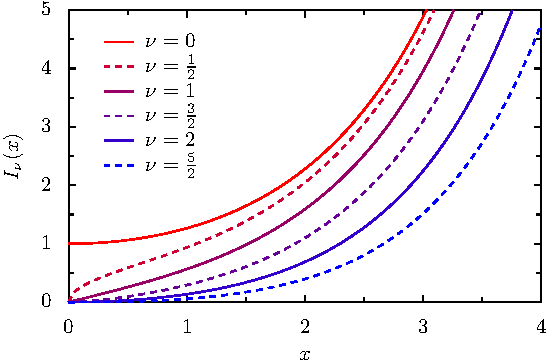
\includegraphics[scale=0.8]{plots/iv.pdf}
    \subcaption{Bessel functions $I_\nu(x)$}
    \end{minipage}%
    \begin{minipage}[b]{.5\linewidth}
    \centering
    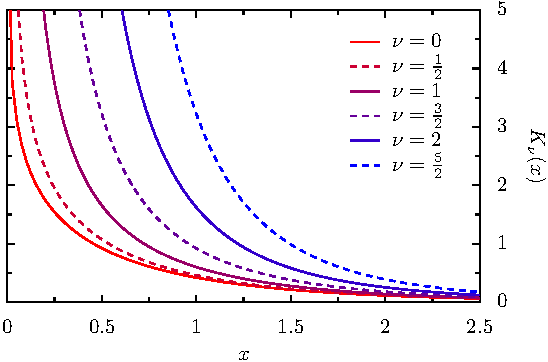
\includegraphics[scale=0.8]{plots/kv.pdf}
    \subcaption{Bessel functions $K_\nu(x)$}
    \end{minipage}

  \caption{Modified Bessel function a) of the first kind and b) of the second kind for various values of $\nu$.}
  \label{fig:appendix_ivkv}
\end{figure}

The modified Bessel functions of the first kind $I_\nu(x)$ and the modified Bessel
function of the second kind $K_\nu(x)$ are defined by
\begin{equation}
I_\nu(x) = \sum_{k=0}^\infty \frac{1}{k! \, \Gamma(k+\nu+1)} \left(\frac{x}{2}\right)^{2k+\nu}, \\
K_\nu(x) = \frac{\pi}{2} \frac{I_{-\nu} (x) - I_\nu (x)}{\sin (\nu \pi)}. 
\end{equation}
The modified Bessel functions satisfy the recurrence relations
\begin{equation}
\label{eq_appendix_bessel_recurrence}
I_{\nu-1}(x) - I_{\nu+1}(x) = \frac{2\nu I_\nu(x)}{x}, \\
K_{\nu+1}(x) - K_{\nu-1}(x) = \frac{2\nu K_\nu(x)}{x}.
\end{equation}
For $\abs{x} \ll 1$ the modified Bessel functions may be approximated by
\begin{equation}
\label{eq:appendix_bessel_approx_small}
I_\nu(x) = \frac{1}{\Gamma(\nu+1)} \left( \frac{x}{2} \right) ^\nu + \mathcal{O}\left(x^{\nu+2}\right), \\
K_\nu(x) = \frac{\Gamma(\nu)}{2} \left( \frac{2}{x} \right) ^\nu + \mathcal{O}\left(x^{\nu+2}\right),
\end{equation}
and for $\abs{x} \gg 1$ by
\begin{equation}
\label{eq:appendix_bessel_approx_large}
I_\nu(x) = \frac{\e^x}{\sqrt{2\pi x}} \left[ 1+\mathcal{O}\left(\frac{1}{x}\right) \right], \\
K_\nu(x) = \sqrt{\frac{\pi}{2x}} \e^{-x} \left[ 1+\mathcal{O}\left(\frac{1}{x}\right) \right].
\end{equation}

Fig. \ref{fig:appendix_ivkv} shows modified Bessel functions of the first and second kind for various values of $\nu$,
Fig. \ref{fig:appendix_ivkv_approx} shows the modified Bessel functions $I_{3/2}$ and $K_{3/2}$, and its approximations.

\begin{figure}
    \begin{minipage}[b]{.5\linewidth}
    \centering
    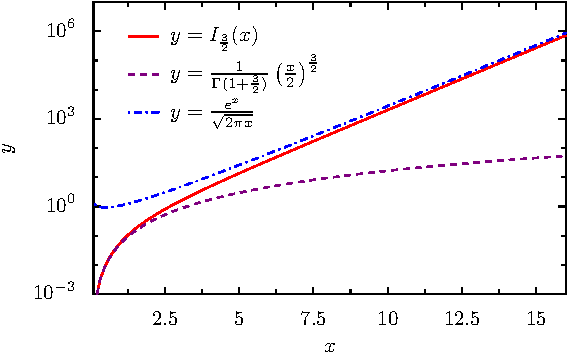
\includegraphics[scale=0.8]{plots/iv_approx.pdf}
    \subcaption{Bessel function $I_3(x)$ and approximations}
    \end{minipage}%
    \begin{minipage}[b]{.5\linewidth}
    \centering
    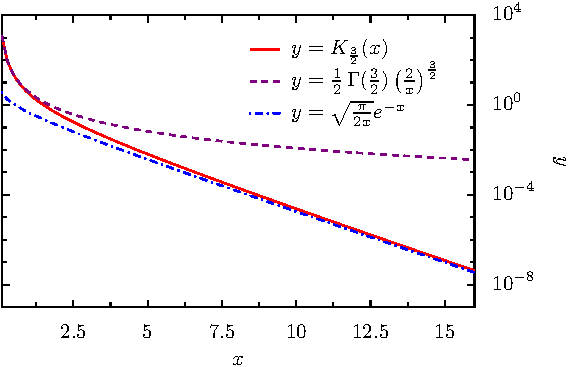
\includegraphics[scale=0.8]{plots/kv_approx.pdf}
    \subcaption{Bessel function $K_3(x)$ and approximations}
    \end{minipage}
  \caption{Bessel functions a) $I_{3/2}(x)$ and b) $K_{3/2}(x)$, and approximations \eqref{eq:appendix_bessel_approx_small} and \eqref{eq:appendix_bessel_approx_large}.}
  \label{fig:appendix_ivkv_approx}
\end{figure}


\section{Polylogarithms}
\label{appendix_polylog}

\begin{figure}
  \begin{center}
      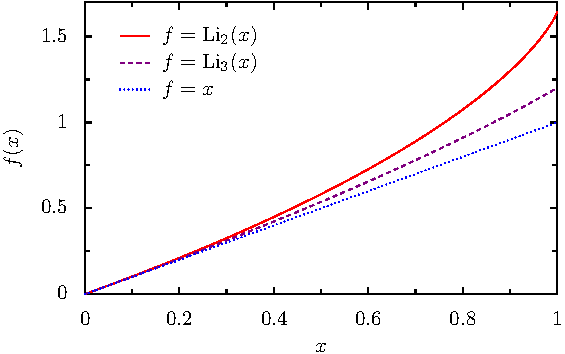
\includegraphics[scale=0.8]{plots/polylog.pdf}
  \end{center}
  \caption{Polylogarithm for $s=2$ and $s=3$.}
  \label{fig:appendix_polylog}
\end{figure}

Polylogarithms are functions that are defined by the power series
\begin{equation}
\label{eq:appendix_polylog_def}
\Li_s(x) = \sum_{k=1}^\infty \frac{x^k}{k^s}
\end{equation}
and depend on a parameter $s$. The series converges for $|x|\le1$.
The polylogarithms for $s=0$ and $s=1$ can be expressed analytically:
\begin{equation}
\Li_0(x) = \frac{x}{1-x} \\
\Li_1(x) = -\log{\left(1-x\right)}
\end{equation}
For integer orders of $s$ polylogarithms can be expressed using the recurrence
formula
\begin{equation}
\Li_{s+1}(x) = \int_0^x \mathrm{d}t \frac{\text{Li}_s(t)}{t}.
\end{equation}
For $x=1$ the polylogarithms reduce to the Riemann zeta function
\begin{equation}
\Li_s(1) = \zeta(s).
\end{equation}
For $x\ll1$ all summands in \eqref{eq:appendix_polylog_def} but $k=1$ can
be neglected and we find the approximation
\begin{equation}
\Li_s \simeq x.
\end{equation}
In Fig. \ref{fig:appendix_polylog} we plot the polylogarithms $\Li_2$ and $\Li_3$.


\chapter{Proofs and mathematical transformations}

\section{Normalization}

\label{appendix_normierung}

In this section, we determine the normalizing constant $A$ 
from the condition
\begin{equation}
\label{eq:appendix_norm1}
\braket{\vec k^\prime, \omega^\prime, \phi^\prime, p^\prime \, | \, \vec k, \omega, \phi, p} \se \delta_{p p^\prime} \, \delta_{\phi \phi^\prime}\, \delta{\left(\vec{k} - \vec{k}^\prime\right)} \, \delta\left(\frac{\omega}{\c}-\frac{\omega^\prime}{\c}\right).
\end{equation}
Inserting the identity operator yields
\begin{align}
\nonumber
&\braket{\vec k^\prime, \omega^\prime, \phi^\prime, p^\prime \, | \, \vec k, \omega, \phi, p} = \int d^3\vec R \, \braket{\vec k^\prime, \omega^\prime, \phi^\prime, p^\prime \, | \, \vec R} \braket{\vec R \, |\,  \vec k, \omega, \phi, p} \\
\nonumber
&\sep =\abs{A}^2 (2\pi)^3 \delta_{p p^\prime} \delta\left(\vec{k}- \vec{k}^\prime\right) \delta\left(\phi k_z- \phi^\prime k_z^\prime\right) \\
\label{eq:appendix_norm2}
&\sep =\abs{A}^2 (2\pi)^3 \delta_{p p^\prime} \delta\left(\vec{k} - \vec{k}^\prime\right) \delta\left(\sqrt{\frac{\omega^2}{\c^2}-k^2}-\frac{\phi^\prime}{\phi}\sqrt{\frac{{\omega^\prime}^2}{\c^2}-k^2}\right),
\end{align}
where we have used that the delta function is even.

In order to cast \eqref{eq:appendix_norm2} in the form of
\eqref{eq:appendix_norm1} we have to rewrite the second delta function. We use
the identity
\begin{equation}
\delta\left(f(x)\right) = \sum_i \frac{\delta\left(x-x_i\right)}{\left|f^\prime(x_i)\right|},
\end{equation}
where $x_i$ are the roots of $f(x)$. We find
\begin{equation}
f\left({\frac{\omega}{\c}}\right) = \sqrt{\frac{\omega^2}{\c^2}-k^2}-\frac{\phi^\prime}{\phi} \sqrt{\frac{{\omega^\prime}^2}{\c^2}-k^2}, \\
f^\prime\left({\frac{\omega}{\c}}\right) = \frac{\omega}{\c \sqrt{\frac{\omega^2}{\c^2}-k^2}} = \frac{\omega}{\c k_z}.
\end{equation}
As $\omega$ and $\omega^\prime$ are non-negative, $f$ has just one
root at $\omega/\c = \omega^\prime/\c$ for $\phi=\phi^\prime$.
For $\phi\ne\phi^\prime$ the function $f$ has no roots and the integral \eqref{eq:appendix_norm2}
vanishes.
We therefore transform the delta function to
\begin{equation}
\label{eq:appendix_delta}
\delta\left(\sqrt{\frac{\omega^2}{\c^2}-k^2}-\frac{\phi^\prime}{\phi}\sqrt{\frac{{\omega^\prime}^2}{\c^2}-k^2}\right) = \delta_{\phi,\phi^\prime} \left|\frac{\c k_z}{\omega}\right| \delta\left(\frac{\omega}{\c}-\frac{\omega^\prime}{\c}\right).
\end{equation}

With \eqref{eq:appendix_delta} eq. \eqref{eq:appendix_norm2} becomes
\begin{align}
\nonumber
\braket{\vec k^\prime, \omega^\prime, \phi^\prime, p^\prime \, | \, \vec k, \omega, \phi, p} &= \abs{A}^2 (2\pi)^3 \delta_{p p^\prime} \, \delta_{\phi,\phi^\prime} \, \delta\left(\vec{k} - \vec{k}^\prime\right) \left|\frac{\c k_z}{\omega}\right| \delta\left(\frac{\omega}{\c}-\frac{\omega^\prime}{\c}\right) \\
\nonumber
&\se \delta_{p p^\prime} \, \delta_{\phi,\phi^\prime}\, \delta{\left(\vec{k} - \vec{k}^\prime\right)} \, \delta\left(\frac{\omega}{\c}-\frac{\omega^\prime}{\c}\right)
\end{align}
and the normalization constant $A$ is given by
\begin{equation}
A = \frac{1}{(2\pi)^{3/2}} \sqrt{\left|\frac{\omega}{\c k_z}\right|}.
\end{equation}
The constant $A$ is only unique up to an arbitrary phase factor. We choose $A$
to be real.

\section{Commutation of $\mathcal{J}_z$ and $\mathcal{M}$}
\label{appendix_conserved_m}

The round-trip operator is invariant under arbitrary rotations around the
$z$-axis, therefore it commutes with the rotation
operator~$\mathcal{R}_z(\varphi)$. The angular momentum operator is the
generator of the rotation and the rotation operator can be expressed as
\begin{equation}
\mathcal{R}_z(\varphi) = \exp{\left( -\imag \varphi \mathcal{J}_z \right)}.
\end{equation}
It is sufficient to consider an infinitesimal rotation, because any finite
rotation can be built from infinitesimal rotations.
For an infinitesimal rotation the rotation operator simplifies to
\begin{equation}
\mathcal{R}_z(\delta\varphi) = \Id - \imag \delta\varphi \mathcal{J}_z
\end{equation}
and we can show that the round-trip operator commutes with the angular momentum
operator
\begin{align}
0 &= \left[\mathcal{R}_z(\delta\varphi), \mathcal{M}\right]
  = \left(\Id - \imag \delta\varphi \mathcal{J}_z\right) \mathcal{M} - \mathcal{M} \left(\Id - \imag \delta\varphi \mathcal{J}_z\right)
  = \imag \delta\varphi \left[\mathcal{M}, \mathcal{J}_z\right] \\
  &\Rightarrow \left[\mathcal{M}, \mathcal{J}_z\right] = 0.
\end{align}
The $z$-component of the angular momentum is thus conserved during
scattering processes, the round-trip operator is block diagonal with respect to
$m$
\begin{equation}
\mathcal{M}(\omega) = \left(\begin{array}{ccccc}
\ddots &                     &                   &                     & 0 \\
       & \mathcal{M}^{(m-1)} &                   &                     & \\
       &                     & \mathcal{M}^{(m)} &                     & \\
       &                     &                   & \mathcal{M}^{(m+1)} & \\
0      &                     &                   &                     & \ddots
\end{array}
\right),
\end{equation}
and each block
$\mathcal{M}^{(m)}$ yields an independent contribution to the free energy
\begin{equation}
\F = \kb T {\sum_{n=0}^\infty}^\prime \log \det \left[\Id - \mathcal{M}(\omega) \right]
       = \kb T {\sum_{n=0}^\infty}^\prime \sum_{m=-\infty}^\infty \log \det \left[\Id - \mathcal{M}^{(m)}(\omega) \right].
\end{equation}



\section{Determinants of block matrices}
\label{appendix_determinant_block_matrices}

Let $A$, $B$, $C$, $D$ $\in \mathbb{C}^{n\times n}$, $\lambda \in \mathbb{C}$, then it follows:
\begin{equation}
\det\left(\begin{array}{cc}
A & \lambda B \\
\frac{1}{\lambda} C & D
\end{array}\right) = 
\frac{1}{\lambda^n} \det\left(\begin{array}{cc}
\lambda A & \lambda B \\
C & D
\end{array}\right) = 
\frac{\lambda^n}{\lambda^n} \det\left(\begin{array}{cc}
A & B \\
C & D
\end{array}\right) = 
\det\left(\begin{array}{cc}
A & B \\
C & D
\end{array}\right)
\end{equation}
In particular, it follows
\begin{equation}
\label{eq:appendix_det_i}
\det\left(\begin{array}{cc}
A & \imag B \\
\imag C & D
\end{array}\right) = 
\det\left(\begin{array}{cc}
A & - B \\
C & D
\end{array}\right)
\end{equation}
and
\begin{equation}
\label{eq:appendix_det_m}
\det\left(\begin{array}{cc}
 A & -B \\
-C &  D
\end{array}\right) = 
\det\left(\begin{array}{cc}
A & B \\
C & D
\end{array}\right)\text{.}
\end{equation}


\section{Equivalence of the matrix elements of \textsc{Canaguier--Durand} et al.}
\label{appendix_umrechnung}

At first glance the matrix elements \eqref{eq:4_EE}--\eqref{eq:4_ME} differ
from those of \textsc{Canaguier--Durand} et al. \cite{Durand,
ThermalCasimirEffect}, but the actual expressions can be rearranged into each
other. We want to demonstrate this for the matrix element
$\mathcal{M}_\TE^{(m)}(E,E)_{\ell_1\ell_2}$.

We start with the matrix element of \textsc{Canaguier--Durand} et al. \cite{Durand, ThermalCasimirEffect}:
\begin{equation}
\mathcal{M}_\TE^{(m)}(E,E)_{\ell_1\ell_2} = \sqrt{\frac{(2\ell_1+1)\pi}{\ell_2(\ell_2+1)}} a_{\ell_1} (-\imag m) \int_0^\infty \frac{\mathrm{d}k}{\kappa} \, \left[ \mathrm{d}^{\ell_1}_{m,1}(\theta^+) + \mathrm{d}^{\ell_1}_{m,-1}(\theta^+)\right] \Ylm{\ell_2,m}(\theta^-,0) \, r_\TE \, \e^{-2\kappa\mathcal{L}}
\end{equation}

We can replace the sum of the Wigner d-matrix elements by an associated Legendre
polynomial using \eqref{eq:appendix_wignerdp}. We also write the spherical harmonic
in terms of an associated Legendre polynomial and get:
\begin{align}
\nonumber
\mathcal{M}_\TE^{(m)}(E,E)_{\ell_1\ell_2} &= \imag m^2 a_{\ell_1} \frac{\sqrt{8} \Nlm{\ell_1 m}}{\sqrt{\ell_2(\ell_1+1)\,(2\ell_1+1)}} \sqrt{\frac{(2\ell_1+1)\,\pi}{\ell_2(\ell_2+1)}} \\
\label{eq:appendix_umformung1}
&\times \int_0^\infty \frac{\mathrm{d}k}{\kappa} \frac{\Plm{\ell_1}{m}\left(\cos\theta^+\right)}{\sin\theta^+} \frac{\Nlm{\ell_2 m}}{\sqrt{2\pi}} \Plm{\ell_2}{m}\left(\cos\theta^+\right) \, r_\TE \, \e^{-2\kappa\mathcal{L}}
\end{align}
Sine and cosine of the Wick rotated polar angle can be expressed by
\begin{equation}
\sin\theta^\pm = \frac{-\imag \c k}{\xi}, \\
\cos\theta^\pm = \pm\frac{\c \kappa}{\xi}.
\end{equation}
After inserting in \eqref{eq:appendix_umformung1}, cancelling and resorting, we find
\begin{align}
\nonumber
\mathcal{M}_\TE^{(m)}(E,E)_{\ell_1\ell_2} &= \imag m^2 a_{\ell_1} \frac{-2 \Nlm{\ell_1 m} \Nlm{\ell_2 m}}{\sqrt{\ell_1(\ell_1+1)\,\ell_2(\ell_2+1)}} \\
&\times \int_0^\infty \frac{\mathrm{d}k}{\kappa} \frac{\xi}{\imag\c k} \, r_\TE \, \Plm{\ell_1}{m}\left(\frac{\kappa\c}{\xi}\right) \Plm{\ell_2}{m}\left(-\frac{\kappa\c}{\xi}\right) \e^{-2\kappa\mathcal{L}}.
\end{align}
This can be rearranged to
\begin{equation}
\label{eq:appendix_umformung2}
\mathcal{M}_\TE^{(m)}(E,E)_{\ell_1\ell_2} = \Lambda_{\ell_1 \ell_2}^{(m)} a_{\ell_1} \frac{m^2\xi}{\c}
\int_0^\infty \mathrm{d}k \frac{1}{\kappa k} \, r_\TE \, \Plm{\ell_1}{m}\left(\frac{\kappa\c}{\xi}\right) \Plm{\ell_2}{m}\left(-\frac{\kappa\c}{\xi}\right) \e^{-2\kappa\mathcal{L}}
\end{equation}
We see that \eqref{eq:appendix_umformung2} is identical to \eqref{eq:4_EE} for the TE mode.


\section{$B_{\ell_1 \ell_2,p}^{(m)}$ for $\xi\to0$}

\label{appendix_integral}

For $\xi=nT\to0$ we may replace $\kappa$ by $k$, because
\begin{equation}
\kappa = \sqrt{n^2T^2+k^2} \overset{nT\to0}{=} k.
\end{equation}
Also, we assume the Fresnel coefficients to be independent of $\xi$ and $k$.
Then, we can put $r_p$ in front of the integral and we obtain
\begin{equation}
B_{\ell_1 \ell_2,p}^{(m)} = \frac{r_p}{(nT)^3} \int_0^\infty \mathrm{d}k \, \e^{-2k} k^2 \Plm{\ell_1}{m}^\prime\left(\frac{k}{nT}\right)\Plm{\ell_2}{m}^\prime\left(-\frac{k}{nT}\right).
\end{equation}
For $nT\to0$ the argument of the associated Legendre polynomials becomes large
according to amount and they can be approximated using
\eqref{eq:appendix_sfun_assoclegendre_dplm_big}:
\begin{equation}
\label{eq:appendix_xi0_a}
B_{\ell_1 \ell_2,p}^{(m)} \simeq r_p \, \frac{(-1)^{\ell_2+m+1}\,(-\imag)^{2m}\,(2\ell_1)!\,(2\ell_2)!}{2^{\ell_1+\ell_2} \, (\ell_1-1)! \, (\ell_2-1)! \, (\ell_1-m)! \, (\ell_2-m)!}
\left(\frac{1}{nT}\right)^{\ell_1+\ell_2+1} \int_0^\infty \mathrm{d}k \, \e^{-2k} \, k^{\ell_1+\ell_2}
\end{equation}
The integral in \eqref{eq:appendix_xi0_a} yields
\begin{equation}
\int_0^\infty \mathrm{d}k \, \e^{-2k} \, k^{\ell_1+\ell_2} = \frac{(\ell_1+\ell_2)!}{2^{\ell_1+\ell_2+1}},
\end{equation}
and after inserting we obtain
\begin{equation}
B_{\ell_1 \ell_2,p}^{(m)} \simeq r_p \, \frac{(-1)^{\ell_2+1} \, (2\ell_1)! \, (2\ell_2)! \, (\ell_1+\ell_2)!}{2^{2\ell_1+2\ell_2+1} \, (\ell_1-1)! \, (\ell_2-1)! \, (\ell_1-m)! \, (\ell_2-m)!}.
\end{equation}
The diagonal block matrices thus become
\begin{align}
\label{eq:appendix_integration_EE}
\mathcal{M}^{(m)}(E,E)_{\ell_1 \ell_2} &\simeq \Lambda_{\ell_1 \ell_2}^{(m)} \, a_{\ell_1} \, B_{\ell_1 \ell_2, \TM}^{(m)} = \Xi_{\ell_1 \ell_2}^{(m)} \, r_\TM^{\xi\to0} \, a_{\ell,0}^\text{perf} \, \left(\frac{R}{\mathcal{L}}\right)^{\ell_1+\ell_2+1} \left(\frac{nT \, R}{\mathcal{L}}\right)^{\ell_1-\ell_2}, \\
\label{eq:appendix_integration_MM}
\mathcal{M}^{(m)}(M,M)_{\ell_1 \ell_2} &\simeq \Lambda_{\ell_1 \ell_2}^{(m)} \, b_{\ell_1} \, B_{\ell_1 \ell_2, \TE}^{(m)} = \Xi_{\ell_1 \ell_2}^{(m)} \, r_\TE^{\xi\to0} \, b_{\ell,0}^\text{perf} \, \left(\frac{R}{\mathcal{L}}\right)^{\ell_1+\ell_2+1} \left(\frac{nT \, R}{\mathcal{L}}\right)^{\ell_1-\ell_2},
\end{align}
where we have defined the prefactor
\begin{equation}
\Xi_{\ell_1 \ell_2}^{(m)} \equiv \Lambda_{\ell_1 \ell_2}^{(m)} \, \frac{(-1)^{\ell_2+1} \, (2\ell_1)! \, (2\ell_2)! \, (\ell_1+\ell_2)!}{4^{2\ell_1+\ell_2+1} \, (\ell_1-1)! \, (\ell_2-1)! \, (\ell_1-m)! \, (\ell_2-m)!}.
\end{equation}
The prefactors $a_{\ell,0}^\text{perf}$ and $b_{\ell,0}^\text{perf}$ have been
defined in \eqref{eq:scattering_ps_mie_prefactors}.

\section{Determinant of $\mathcal{M}^{(m)}(P,P)$ for $\xi\to0$}

\label{appendix_det}

For $n=0$ the Matsubara frequency $\xi_{n=0}=nT=0$ vanishes.
The matrix elements scale
as $\mathcal{M}^{(m)}(P,P)_{l_1 l_2} \sim \lambda^{\ell_1-\ell_2}$, where
\begin{equation}
\lambda = \frac{nT \, R}{\mathcal{L}},
\end{equation}
and the matrix looks like
\begin{equation}
\mathcal{M}^{(m)}(P,P) = \left(
\begin{array}{cccc}
a_{11}\,\lambda^{0}      & a_{12}\,\lambda^{-1}        & \cdots & a_{1n}\,\lambda^{-n+1}  \\
a_{21}\,\lambda^{1}      & a_{22}\,\lambda^{0}         & \cdots & a_{2n}\,\lambda^{-n+2}  \\
\vdots               &                      & \ddots   & \vdots              \\
a_{n-1,1}\,\lambda^{n-2} & a_{n-1,2}\,\lambda^{n-3}    & \cdots & a_{n-1,n}\,\lambda^{-1} \\
a_{n1}   \,\lambda^{n-1}    & a_{n2}\,\lambda^{n-2}    & \cdots & a_{nn}   \,\lambda^{0} 
\end{array}
\right),
\end{equation}
where $a_{ij}$ are coefficients that are independent of $\lambda$.

Let us multiply the first row of the matrix by the factor $\lambda^{n-1}$,
the second row by the factor $\lambda^{n-2}$, $\cdots$, and the second last
row by the factor $\lambda^1$.
As the determinant of a $n\times n$ matrix is a $n$-linear function,
multiplying a row or a column by a factor $\alpha$ alters the determinant by
a factor $\alpha$.
So we have to multiply $\lambda^{-1}\lambda^{-2}\dots\lambda^{-n+1}$
in order to keep the value of the determinant constant:
\begin{equation}
\det \mathcal{M}^{(m)}(P,P) = \prod_{k=1}^{n-1} \lambda^{-k} \det\left(
\begin{array}{cccc}
a_{11}\,\lambda^{n-1}    & a_{12}\,\lambda^{n-2}    & \cdots & a_{1n}\,\lambda^0    \\
a_{21}\,\lambda^{n-1}    & a_{22}\,\lambda^{n-2}    & \cdots & a_{2n}\,\lambda^0    \\
\vdots               &                      & \ddots & \vdots           \\
a_{n-1,1}\,\lambda^{n-1} & a_{n-1,2}\,\lambda^{n-2} & \cdots & a_{n-1,n}\,\lambda^0 \\
a_{n1}\,\lambda^{n-1}    & a_{n2}\,\lambda^{n-2}    & \cdots & a_{nn}\,\lambda^0
\end{array}
\right)
\end{equation}
If we now multiply the first column by the factor $\lambda^{n-1}$, the second column by 
the factor $\lambda^{n-2}$, $\dots$, and the second last column by the factor $\lambda$, the
prefactor vanishes and we obtain:
\begin{equation}
\det \mathcal{M}^{(m)}(P,P) = \det\left(
\begin{array}{cccc}
a_{11} & a_{12} & \cdots & a_{1n} \\
a_{21} & a_{22} & \cdots & a_{2n} \\
\vdots &        & \ddots & \vdots \\
a_{n-1,1} & a_{n-1,2} & \cdots & a_{n-1,n} \\
a_{n1} & a_{n2} & \cdots & a_{nn}
\end{array}
\right)
\end{equation}

For this reason, the determinant is independent of $\lambda$ and thus
also independent of $\xi=nT$.


\section{Infinite series}

For $|q|<1$ the value of the geometric series is:
\begin{equation}
\label{appendix_geom_series}
\sum_{k=0}^\infty q^k = \frac{1}{1-q}
\end{equation}
By differentiating the left and right hand side of
\eqref{appendix_geom_series}, and multiplying by $q$, we obtain:
\begin{equation}
\label{appendix_geom_series_k}
\sum_{k=0}^\infty kq^k = \frac{q}{(1-q)^2}
\end{equation}
Silmilarly, differentating two times and multiplying by the factor $q^2$ yields:
\begin{equation}
\label{appendix_geom_series_k2}
\sum_{k=0}^\infty k^2 q^k = \frac{2q^2}{(1-q)^2} + \sum_{k=0}^\infty kq^k = \frac{q(q+1)}{(1-q)^3}
\end{equation}


\section{Scattering at a sphere and factor $-2$}
\label{appendix_factor2}

The matrix elements for the scattering at the sphere are given by
\begin{align}
\label{eq:appendix_mie_a}
\braket{\ell,m,E \, | \, \mathcal{R}_\text{S} \, | \, \ell,m,E} &= -2 a_\ell(\omega), \\
\label{eq:appendix_mie_b}
\braket{\ell,m,M \, | \, \mathcal{R}_\text{S} \, | \, \ell,m,M} &= -2 b_\ell(\omega).
\end{align}
However, the appearance of the factor $-2$ is contrary to expectation.
In this section, we will discuss the reason for the appearance of the factor $-2$.
The scattering of plane waves at a sphere is discussed in Refs. \cite{jackson, kerker},
however, we will only refer to \cite{bohrenhuffman} in our argumentation.

The problem of absorption and scattering of electromagnetic waves at a sphere
is usually called Mie scattering in literature. Usually, one considers
a plane $x$-polarized wave that propagates in $+z$-direction. Arbitrary
incident angles and polarizations may be described by a rotation of the
coordinate system using Wigner-D matrices \cite{biedenharn, rose}.

The incident plane wave may be expanded in VSH
\begin{equation}
\label{eq:appendix_f2_entw}
\vec E_\text{i}(\vec R) = \sum_{\ell=1}^\infty E_\ell \left(\vec M_{\text{o}, \ell 1}^{(1)} - \imag \vec N_{\text{e}, \ell 1}^{(1)} \right), \\ E_\ell = \imag^\ell E_0 \frac{2\ell+1}{\ell(\ell+1)},
\end{equation}
where $E_0$ corresponds to the amplitude of the incident wave, $\vec M$
and $\vec N$ are VSH. These VSH, however, differ from the VSH we introduced
in section \ref{chapter_basis_multipol}. The VSH $\vec M$ and
$\vec N$ are defined in real space and have a radial dependence. The
superscript ``1'' denotes that the radial dependence is given by
spherical Bessel functions $j_\ell$. Moreover, the VSH $\vec M$ and $\vec N$
are separated in even (e) and odd (o) functions, and the value of $m$
is non-negative. In the expansion \eqref{eq:appendix_f2_entw} all terms
but $m \ne 1$ vanish.

The expansion of the scattered wave is given by
\begin{equation}
\label{eq:appendix_f2_entw2}
\vec E_\text{s}(\vec R) = -\sum_{\ell=1}^\infty E_\ell \left(b_\ell \vec M_{\text{o}, \ell 1}^{(3)} - \imag a_\ell \imag \vec N_{\text{e}, \ell 1}^{(3)} \right),
\end{equation}
where the superscript ``3'' denotes that the radial dependence is given
by spherical Hankel functions of the first kind $h_\ell^{(1)}$.

Comparing \eqref{eq:appendix_f2_entw} and \eqref{eq:appendix_f2_entw2}
reveals that the sign in the matrix elements \eqref{eq:appendix_mie_a} and
\eqref{eq:appendix_mie_b} is caused by the definition of the Mie coefficients:
\begin{align}
\label{eq:appendis_f2_ew1}
\mathcal{R}_\text{S} \vec{N}_{\text{o},\ell 1}^{(1)} &= -a_\ell \vec{N}_{\text{o},\ell 1}^{(3)} \\
\label{eq:appendis_f2_ew2}
\mathcal{R}_\text{S} \vec{M}_{\text{o},\ell 1}^{(1)} &= -b_\ell \vec{M}_{\text{o},\ell 1}^{(3)}
\end{align}
However, the reason of the factor $2$ is still unclear. Eqs. 
\eqref{eq:appendis_f2_ew1} and \eqref{eq:appendis_f2_ew2} are no
eigenvalue equations, because the radial dependence for the incident
and the scattered fields are different: The radial dependence of the
incident wave is given by spherical Bessel functions $j_\ell$, while
the radial dependence of the scattered wave is given by spherical Hankel functions of the
first kind $h^{(1)}_\ell$. So, the Hankel functions
$h^{(1)}_\ell$ have to be converted to spherical Bessel functions $j_\ell$.
This is possible for different origins and the factor $2$ is due to this
conversion \cite{bostroem}. 

A derivation of the formulae in real-space is carried out in
\cite{PhysRevA.92.062504}.
